% Chapter 1

\chapter{Introducción} % Chapter title

\label{ch:introduccion} % For referencing the chapter elsewhere, use \autoref{ch:introduccion} 
\lhead{\emph{Introducción}} % Change X to a consecutive number; this is for the header on each page - perhaps a shortened title

%----------------------------------------------------------------------------------------
En este capítulo se dará una breve introducción a la problemática a resolver. Las siguientes secciones tratarán la motivación,
la definición del problema a trabajar y el plan de tesis.

\section{Contexto}
    
Las antenas de arreglo de fase controlada \cite{Fenn2000} son utilizadas en aplicaciones de todo tipo, por ejemplo comunicaciones 
de móviles \cite{Chen2012}, aéreas \todo{encontrar la siguiente cita entre las cosas del mendeley}
								   \cite{ppr:punc-ext1} y espaciales \cite{Shimada1995}\cite{Makhoul2012}. 

Para generar diversos productos, por ejemplo imágenes satelitales en radares SAR \todo{encontrar la siguiente cita entre las cosas del mendeley}
																				 \cite{ppr:puncTrgt1}, es necesario que estén 
correctamente calibradas \todo{encontrar la siguiente cita entre las cosas del mendeley}
						 \cite{ppr:classic1}\cite{ppr:classic2}\cite{ppr:classic3}. Esto implica, que las tolerancias de
fases y amplitudes se mantengan en el tiempo y/o sus valores sean bien conocidas
para cada elemento del arreglo.

Generalmente, este tipo de antenas son calibradas en tierra utilizando fuentes 
externas de campo lejano o cercano [\ref{ppr:mutual1}]. Sin embargo, en 
aplicaciones aéreas o espaciales, la utilización de dichas fuentes es impráctica
o difícil de implementar [\ref{ppr:mutual3}]. Resulta fundamental un esquema de
calibración interna que permita tener bajo control estas variables. Generalmente
se implementan lazos de calibración internos [\ref{ppr:classic1}]
[\ref{ppr:classic2}][\ref{ppr:classic3}][\ref{ppr:abs-rad-ical1}]
[\ref{ppr:classic4}][\ref{ppr:classic5}][\ref{ppr:classic6}]
[\ref{ppr:classic-ext1}][\ref{ppr:classic7}]\cite{Makhoul2012}. 
Luego se opta por caracterizar todos aquellos componentes que no entran dentro 
de dicho lazo de calibración [\ref{ppr:abs-rad-ical1}].
Este método presenta algunos inconvenientes. Por dar un par de ejmplos se puede
mencionar que los recursos necesarios (tiempo, personal) durante la campaña de 
ensayos previa al lanzamiento impactan en todo el desarrollo de actividades, o
que las consecuencias que puede traer el hecho de que la caracterización no sea
válida porque un determinado componente envejece con el paso del tiempo.

En este contexto, se investiga y propone un método que permita reducir costos 
asociados a la calibración y por ende a los proyectos:

\begin{enumerate}
    \item Evitando la necesidad de realizar caracterizaciones previas de la 
antena de arreglo de fase.
    \item Permitiendo conocer en tiempo real, y para el estado real de la antena
, los valores reales de fase y amplitud en vuelo que transmite la antena, 
independientemente de su estado de envejecimiento.
\end{enumerate}

En este sentido se investiga y aprovecha el concepto acoplamiento mutuo 
inherente entre los módulos radiantes de la antena [\ref{ppr:mutual3}], pero de
manera complementaria al enfoque tradicional. 

En esta tesis se realizarán las siguientes tareas:

\begin{enumerate}
    \item Se explicarán las ventajas y desventajas del método propuesto respecto
del tradicional.
    \item Se analizarán y propondorán los requerimientos para poder 
implementarlo.
    \item Se desarrollará un modelo de antena de arreglo de fase polarimétrico 
básico representativo en parámetros S \ref{pr:parameters}.
    \item Se añadirán al mismo parámetros de dispersión de comportamiento que 
permitan analizar su comportamiento.
    \item Se realizará un modelo de calibración que será implementado 
algoritimicamente.
\end{enumerate}


\section{Definiciones}

{\textbf{Antena de arreglo de fase}} (en inglés: phased array) es un conjunto de antenas en que las fases relativas de las 
señales con que se alimenta cada antena se varían intencionadamente con objeto de alterar el diagrama de radiación del 
conjunto. Lo normal es reforzar la radiación en una dirección concreta y suprimirla en direcciones indeseadas. Si todos los 
elementos del arreglo de fase están contenidos en el mismo plano y la señal con que se alimentan es de la misma fase, 
entonces se estará reforzando la dirección perpendicular a ese plano. Si se altera la fase relativa de las señales se podrá
\enquote*{mover} el haz (en realidad lo que se está haciendo es cambiar la dirección en la cual las interferencias son 
constructivas). Se consigue de este modo hacer barridos sin necesidad de movimiento físico, con la ventaja añadida de que 
se pueden barrer ángulos del orden de miles de grados por segundo. Esto permite utilizar la antena para compaginar 
simultáneamente funciones de detección y de seguimiento muchos blancos individuales, asi como para obtener imágenes de 
apertura sintética. Su uso se va extendiendo debido a la confiabilidad derivada del hecho de que no tienen partes móviles. 
Casi todos los radares militares modernos se basan en phased arrays, relegando los sistemas basados en antenas rotatorias a 
aplicaciones donde el costo es un factor determinante (tráfico aéreo, meteorología, etc) Su uso está también extendido en
aeronaves militares debido a su capacidad de seguir múltiples objetivos. El primer avión en usar uno fue el B-1B Lancer, y 
el primer caza, el MiG-31 ruso.\\

{\textbf{Calibración interna}} es colocar sensores que permitan la medición directa u indirecta de los distintos parámetros 
del sistema en vuelo. 

Estas mediciones obtenidas con este sistema son útiles solamente al utilizarlas en conjuto a los resultados de los test 
realizados en tierra, los cuales definen la relación entre lo observado y la performance de los párametros del sistema. 
Ejemplos de satélites para los cuales se utilizó calibración interna son el E-ERS-1 y el SIR-C.
    
Los tests realizados en tierra para dichos sistemas complejos son sobre la electrónica de RF, la electrónica digital y la 
antena sobre temperatura; para los cuales es preferible realizarlos, cuando sea posible, en un ambiente al vacío. Los 
parámetros clave del sistema, como: potencia transmitida, pérdidas de transmisión o recepción, ganancia de recepción, 
ganancia y patrón de la antena, linealidad de la electrónica digital/RF, rango dinámico, y fase/amplitud vs estabilidad de la 
frecuencia son medidos en función de la temperatura para cada seteo de ganancia del radar y PRF (Pulse Repetition Frequency). 
Los elementos de calibración, como medidores de temperatura, de corriente y de potencia, podrán permitir la determinación de 
la performance del sistema en función de la variación de dichos parámetros.
    
Esta técnica asume que la variación en la performance del sistema puede ser modelada en función de los parámetros observables. 
También, se asume que los componentes de calibración están correctamente calibrados y son estables en el paso del tiempo. 
Además de estos tests, en la mayoría de los sistemas de radar se realizan mediciones de componentes de RF utilizando loops de 
calibración.
	

\section{Motivación}

A la hora de adquirir imágenes satelitales es crucial que se conozca perfectamente la señal emitida y recibida por la antena. 
Ya sea por envejecimiento de los componentes [\ref{ppr:mutual1}] o por variaciones de temperaturas se observan dispersiones de 
las mismas [\ref{ppr:sim1}]. 

El método de calibración tradicional, por lazos de calibración internos, permite calibrar una antena de arreglo de fase, aunque 
adolece de algunos defectos entre los cuales se incluyen:

\begin{enumerate}
    \item Una degradación o directamente rotura de un elemento radiante, el cual está fuera del lazo de calibración interno, no 
			es detectado por la calibración interna.
    \item Existen elementos que quedan fuera del lazo de calibración interno. Como por ejemplo los circuladores. Esto lleva a 
			la necesidad de realizar caracterizaciones en tierra lo cual implica consumo de recursos de proyecto importantes, 
			además de tener que confiar que dicha caracterización será válida (o sea que no habrá envejecimiento de los mismo) 
			luego durante vuelo en toda la vida útil de la antena.
    \item Cada lazo de calibración no se interrelaciona con el resto haciendo que no se pueda disminuir el error de medición por 
			multiplicidad de caminos.
\end{enumerate}

Esto lleva a investigar opciones superadoras, que den lugar a un método de calibración que permita complementar al tradicional 
evitando la necesidad de realizar costosas caracterizaciones en tierra, previendo que los componentes en vuelo puedan envejecer 
y por ende dichas caracterizaciones no ser más validas, permitiendo detectar fallas en elementos que en la calibración interna 
tradicional quedan fuera del lazo de calibración, y disminuyendo la incertidumbre en la determinación de la fase y amplitud de 
salida.

El método que se propone en esta tesis, denominado de \enquote*{método de calibración interna complementada por acoplamientos 
mutos (MCINCAM)} toma la idea de mediciones por acoplamiento mutuo [\ref{ppr:mutual1}][\ref{ppr:mutual2}] [\ref{ppr:mutual3}]
[\ref{ppr:mutual-ext1}], para integrarla de manera complementaria al método tradicional, sin necesidad de agregar hardware 
adicional, y además establece los requerimientos electrónicos para poder implementarla. En esta tesis además se realiza un modelo 
ad hoc, en parámetros S, de antena, para mostrar la eficacia del método. 


\section{Objetivo de la Tesis}

La presente tesis tiene varios objetivos:

\begin{enumerate}
    \item Presentar conceptualmente el método tradicional de calibración interna de una antena polarimétrica que abarque el 
			sistema completo de transmisión/recepción. con sus virtudes y defectos. Mencionar algunas misiones de ejemplo en
			las cuales el mismo se ha utilizado.
    \item Investigar, desarrollar y presentar conceptualmente un método alternativo de calibración interna que introduzca 
			mejoras al método tradicional sin necesidad de introducir hardware adicional y con la premisa fundamental de 
			reducir los costos asociados a las caracterizaciones que el método tradicional incluye. Introducir los 
			requerimientos necesarios para poder implementarlo.
    \item Investigar, desarrollar y presentar (generar) los algoritmos que permitan representar el modelo de antena 
			polarimétrico (modelo de capa física) que serán utilizados para poder comparar el método tradicional y el 
			alternativo. Dichos modelos deben representar el comportamiento en RF básico de las señales al propagarse por el 
			sistema.
    \item Generar los algoritmos que permitan correr el algoritmo de calibración alternativo de manera de poder comparar ambos 
			métodos.
    \item Sacar conclusiones respecto a los pros y contras del método propuesto, en particular en referencia al método 
			tradicional, por medio de algunos parámetros objetivos como ser tiempo de calibración, caracterizaciones necesarias, 
			incertidumbre de medición, entre otros.
\end{enumerate}    


\section{Especificaciones del problema}

\begin{itemize}
    \item La aplicación debera reproducir el comportamiento en RF de los elementos individuales: cables, psc, TRM, elementos 
			radiantes.

    \item La aplicación deberá reproducir el comportamiento del sistema el cual será LTI (lineal e invariante en el tiempo).
    
    \item La antena debe estar compuesta por defasadores, atenuadores, cables, divisores de potencia y módulos radiantes.
    
    \item Se deben poder utilizar distintos divisores/combinadores de potencia. La diferencia entre ellos es la cantidad de 
			puertos de salida.
    
    \item Los componentes de la antena deben caracterizarse utilizando parámetros de alta frecuencia.
    
    \item Se debe tener en cuenta el efecto que impone un componente al resto de la antena.

    \item Se debe poder configurar la dimensión de la antena.
    \item Se debe poder configurar la distancia entre elementos radiantes.
    \item Se debe poder configurar los atributos que afecten la modelización de cada componente de la antena. 
    
    \item Se debe poder configurar el largo de los cables.
    \item Se debe poder configurar la atenuación de los cables.
    
    \item Se debe poder configurar el error de comportamiento de cada componente de la antena de forma independiente.

    \item Se deben poder configurar los atenuadores y defasadores a la hora de realizar la calibración. 

    \item La aplicación debe poder calibrar una antena polarimétrica con el método de calibración convencional.
    
    \item La aplicación debe poder calibrar una antena polarimétrica con el método de calibración alternativo.
    
    \item La aplicación debe poder calibrar la potencia de transmisión y recepción.
    
    \item La aplicación debe poder calibrar la fase de transmisión y recepción.
    
    \item La aplicación debe poder calibrar en ambas polarizaciones: horizontal y vertical.
    
    \item Se debe poder alcanzar el estado de calibración deseado partiendo cualquier estado inicial en los defasadores y 
			atenuadores.
    
    \item No se puede calibrar en la misma polarización transmisión y recepción a la vez.
    
    \item La antena tiene que ser perfectamente plana. No deben haber imperfecciones.
           
    \item Se debe poder configurar la frecuencia de trabajo.

    \item Se debe poder configurar los parámetros de error (desvío estandar) para la ganancia y fase de la chirp utilizada 
			entre pulsos.

    \item Se debe poder configurar los parámetros de error (desvío estandar) para la ganancia y fase de la chirp réplica 
			utilizada a la hora de realizar la calibración convencional.
    
    \item Se debe poder configurar los parámetros de error (desvío estandar) para la fase de la codificación utilizada a la 
			hora de realizar la calibración convencional.

    \item Se debe poder simular, configurar la destrucción total de elementos de la antena SAR como ser los TRMs.
\end{itemize}


\section{Metodología de la tesis}
\todo{cambiar la forma con que esta escrito esto}
En la presente tesis se investigarán los métodos de calibraciones actuales para poder determinar que ventajas, desventajas, 
limitaciones y diferencias hay entre cada una de ellos. Se buscará tener una visión global de esta problemática para poder 
determinar y entender que posibles falencias puede tener este método alternativo.

Posteriormente, se investigarán las limitaciones que poseen las antenas polarimétricas para poder determinar que recaudos 
se deben tener en cuenta a la hora de desarrollar el método.

Luego, tomando todo en cuenta, se determinarán las hipótesis necesarias para que el algoritmo funcione correctamente. Para 
la validación del método se realizará un modelo de antena.

Finalmente, se probarán, analizarán y documentarán los resultados obtenidos de la comparación entre el algoritmo propuesto 
y el algoritmo de la calibración convencional. A su vez, se dejará asentado que posibles mejoras se podrían aplicar al 
algoritmo para determinar otros aspectos que están fuera del alcance de esta tesis.



\section{Contribución}

En el presente trabajo se presenta una metodología de 


\section{Estructura de la Tesis}

Los siguientes capítulos se organizan de la siguiente manera: se planteará la problemática de la calibración de una antena
polarimétrica en el siguiente capítulo. En el capítulo 3 se formula en detalle los distintos aspectos a considerar al 
trabajar con la calibración. En el capítulo 4, se detallan los trabajos relacionados al presente problema. En el capítulo 5,
se explicará el método que se plantea para resolver \textbf{esta} mierda \todo{corregir y sacar}. En el capítulo 6 se 
describe el desarrollo de la propuesta, seguido por el capítulo 7 con la experimentación (o modelización). Finalmente, se presentarán las 
conclusiones en el capítulo 8.

\todo{todo}
\section{Presentación previa de este trabajo}
\todo{todo}


\begin{comment}
Desde hace algún tiempo se ha estado gestando un gran interés por el desarrollo de las energías alternativas, motivado por la búsqueda
de fuentes eficientes, duraderas y poco contaminantes que podrían reemplazar las fuentes energéticas convencionales.
Dentro de ellas se cuentan principalmente la energía hidráulica, eólica y solar. Una de las desventajas de las mencionadas frente a los
combustibles es la posibilidad de ser almacenados para su disponibilidad inmediata. Sin embargo, existen también combustibles limpios,
como el \textbf{hidrógeno}.

El hidrógeno es un combustible de alto contenido energético y obtenible mediante diversos procesos, cuya reacción con el oxígeno produce agua
limpia. Estas características lo convierten en una opción atractiva frente al resto de los combustibles, tales como los hidrocarburos.

La utilización del hidrógeno como combustible para la generación de energía eléctrica se puede dar de varias maneras. Si bien su combustión
directa es una forma de obtener energía calórica que puede transformarse mediante procesos de conversión habituales, también puede conseguirse
energía eléctrica directamente usando mecanismos electroquímicos. Un modo de hacer esto es mediante \textbf{Celdas de combustible}.

\section{Celdas de combustible}
Las celdas de combustible son dispositivos electroquímicos que permiten obtener energía eléctrica a partir de la reacción química controlada
entre un combustible y un oxidante. Algunos de sus beneficios son su gran eficiencia comparada con las máquinas térmicas convencionales y
las reducidas emisiones de los procesos puestos en juego. Su utilización aún no es muy amplia debido a su elevado costo y la limitada
disponibilidad de los combustibles empleados.

Existen diversos tipos de celdas de combustible, aunque este trabajo solo se ocupa de las celdas de membrana de intercambio protónico
(PEM, por sus siglas en inglés), que operan a bajas temperaturas entregando potencia reducida. 

El uso práctico de las celdas comprende la disposición de varios elementos que forman un sistema. Por un lado, debido al reducido nivel
de tensión que entregan las celdas, suelen utilizarse arreglos de celdas en serie de modo que se obtenga un nivel adecuado de tensión entre
los electrodos terminales. Tales arreglos son llamados pilas de combustible. Por otro lado, durante la operación de las pilas se producen
fenómenos físicos, térmicos, electroquímicos, eléctricos, entre otros. Esto deriva en la necesidad de un sistema compuesto por un conjunto
de elementos auxiliares que tengan en cuenta los efectos de estos fenómenos sobre el comportamiento de la pila.

\section{Sistemas de generación híbridos}
Más allá de todas las ventajas mencionadas acerca de las celdas de combustible se han comentado varias de sus dificultades. La necesidad de
producir el combustible que consumen hace que pierdan autonomía. Es por ello que se ha sugerido su utilización en el contexto de los que se conocen 
como \textit{sistemas de generación híbrida} (SGH), cuyos módulos de generación extraen energía de diferentes fuentes. El presente trabajo 
se enmarca en el diseño de uno de estos sistemas, que en particular está compuesto por fuentes de energías limpias. En la fig. \ref{fig:sist_hibrido}
se muestra el esquema del sistema para el cual fue realizado este proyecto.

\begin{figure}[H]
 \centering
 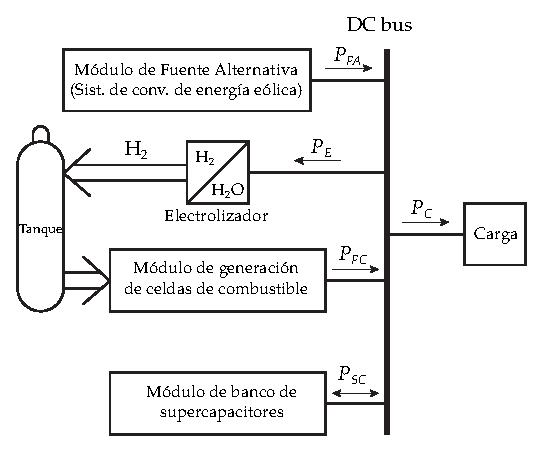
\includegraphics{gfx/diagrama_bloques_sistema_hibrido.eps}
 \caption{Diagrama en bloques de sistema híbrido}
 \label{fig:sist_hibrido}
\end{figure}

Para poder encarar la concepción del SGH se necesitarían todos los módulos que lo componen, esto representaría un gran costo. Por ello se ha
planteado una alternativa para el armado del sistema que consiste en la temporal sustitución de los módulos faltantes por plataformas de emulación.

\section{Emulador de pila de combustible}
El trabajo que se expone en el presente documento trata sobre el diseño y construcción de un emulador de pilas de combustible.
La necesidad del desarrollo de un emulador de pilas de combustible surge a partir de las diversas dificultades para obtener una pila
real, ya sea por su costo, su tamaño o el difícil acceso y almacenamiento del combustible.

La conexión de los módulos mostrados en la fig. \ref{fig:sist_hibrido} hacia el bus de tensión continua debe realizarse mediante una etapa de potencia 
que adapte los niveles eléctricos. En el proyecto del SGH, esta tarea ya ha sido abordada y constituyó el soporte para el desarrollo del emulador. 
La etapa de potencia consiste en un convertidor DC-DC conmutado elevador.

El flujo de trabajo del proyecto se llevó a cabo  de la siguiendo las tareas que se mencionan a continuación: en primer instancia se diseñaron los modelos
de simulación que luego fueron programados en el \emph{hardware} de control y se procedió a la realización de ciertos ajustes en la placa diseñada para el 
convertidor original cambiando la topología del mismo para permitirle funcionar según los modelos diseñados para finalmente realizar los ensayos finales.
\end{comment}
